\documentclass[10pt]{article}
\usepackage{tikz}
\usepackage[margin=0cm]{geometry}
\pagestyle{empty}

\begin{document}

\vspace*{\fill}
\begin{center}
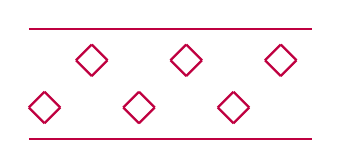
\begin{tikzpicture}[x=0.2cm, y=-0.2cm, thick, purple]
% North to South lines
% North-West to South-East lines
    \draw (4,1) -- (5,2);
    \draw (10,1) -- (11,2);
    \draw (16,1) -- (17,2);
    \draw (3,2) -- (4,3);
    \draw (9,2) -- (10,3);
    \draw (15,2) -- (16,3);
    \draw (1,4) -- (2,5);
    \draw (7,4) -- (8,5);
    \draw (13,4) -- (14,5);
    \draw (0,5) -- (1,6);
    \draw (6,5) -- (7,6);
    \draw (12,5) -- (13,6);
% West to East lines
    \draw (0,0) -- (18,0);
    \draw (0,7) -- (18,7);
% South-West to North-East lines
    \draw (3,2) -- (4,1);
    \draw (9,2) -- (10,1);
    \draw (15,2) -- (16,1);
    \draw (4,3) -- (5,2);
    \draw (10,3) -- (11,2);
    \draw (16,3) -- (17,2);
    \draw (0,5) -- (1,4);
    \draw (6,5) -- (7,4);
    \draw (12,5) -- (13,4);
    \draw (1,6) -- (2,5);
    \draw (7,6) -- (8,5);
    \draw (13,6) -- (14,5);
\end{tikzpicture}
\end{center}
\vspace*{\fill}

\end{document}
